\begin{frame}{Todo es acerca de la conveniencia}
    \centering
    \begin{tikzpicture}
        \node at (1.4,7) {\tiny \bf {Usuario de SGBD}} ;
        \node[inner sep=0pt] at (1.4,5.8) {
            
\includegraphics[width=1.8cm]{img/hface.png}
        };

        \node at (1.4,4.3) {\tiny \bf {Desarrollador de SGBD}} ;
        \node[inner sep=0pt] at (1.4,3.2) {
            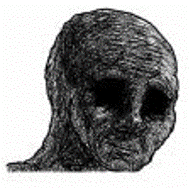
\includegraphics[width=1.8cm]{img/sface.png}
        };

        \draw[-,thick] (0.3, 4.6) -- (7,4.5);
        \draw[-,thick] (2.7, 2) -- (2.7,7.4);

        \onslide<1>{
        \node at (5,5.8) {Lenguaje declarativo};
        \node at (5,4.3) {Estructuras de datos};%\\Algoritmos\\Optimizaci\'on\\Compilaci\'on\\Gesti\'on de ficheros};
        \node at (5,3.8) {Algoritmos};%\\Algoritmos\\Optimizaci\'on\\Compilaci\'on\\Gesti\'on de ficheros};
        \node at (5,3.3) {Optimizaci\'on};%\\Algoritmos\\Optimizaci\'on\\Compilaci\'on\\Gesti\'on de ficheros};
        \node at (5,2.8) {Compilaci\'on};%\\Algoritmos\\Optimizaci\'on\\Compilaci\'on\\Gesti\'on de ficheros};
        \node at (5,2.3) {Gesti\'on de ficheros};%\\Algoritmos\\Optimizaci\'on\\Compilaci\'on\\Gesti\'on de ficheros};
        }

        \onslide<2>{
            \node at (5.3,5.8) {Modelo matem\'atico de datos};
            \node at (5,3) {Implementaci\'on};%\\Algoritmos\\Optimizaci\'on\\Compilaci\'on\\Gesti\'on de ficheros};

        }
    \end{tikzpicture}


\end{frame}

{
\setbeamertemplate{background} 
{
    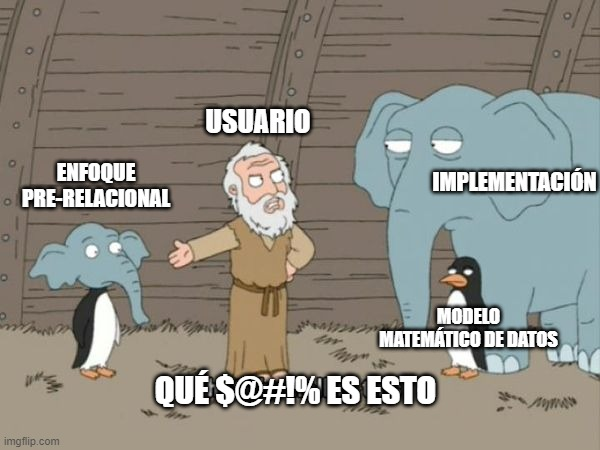
\includegraphics[width=\paperwidth,height=\paperheight]{img/prerelational.jpg}
}
\begin{frame}
\end{frame}
}

\begin{frame}{Enfoques pre-relacionales}
    \vspace{5mm}
    \begin{overlayarea}{\linewidth}{\textheight}
        
        \begin{block}<1->{Importancia}
            \begin{itemize}
                \item Fueron las primeras soluciones computacionales capaces de almacenar y consultar grandes conjuntos de datos.
                \item Se desarrollaron productos comerciales de larga vida basados en estos sistemas.
            \end{itemize}
            
        \end{block}
    
        \begin{block}<2->{Problemas}
            \begin{itemize}
                \only<2>{
                \item Los modelos de datos se consideran como abstracciones de
                las estructuras de almacenamiento subyacentes en el nivel
                físico y sus operadores asociados.}
                \item<3-> El modelo depend\'ia de la implementaci\'on.
                \only<4>{
                \item Los datos se representan por colecciones de registros
                (\textit{records}) y las interrelaciones entre los datos se representan
                mediante enlaces (\textit{links}).}
                \item<5-> Eran muy complicados de utilizar.
                \item<6-> Los usuarios son programadores que se deben encargar, incluso, de la optimizaci\'on.
    
            \end{itemize}
        \end{block}
    \end{overlayarea}
\end{frame}


\begin{frame}{Modelos jer\'arquico y reticular}
    \begin{columns}
        \begin{column}[t]{.5\textwidth}
            \begin{block}{Modelo jer\'arquico}
                \begin{itemize}[<+->]
                \item Las interrelaciones se representan como jerarqu\'ias.
                \item Ning\'un hijo puede existir sin su padre.
                \item Se recorre un \'arbol para: \textcolor<7>{red}{insertar}, \textcolor<7>{red}{actualizar}, \textcolor<7>{red}{eliminar} y \textcolor<7>{red}{buscar}.
                \end{itemize}
            \end{block}
        \end{column}

        \begin{column}[t]{.5\textwidth}
            \begin{block}<4->{Modelo reticular}
                \begin{itemize}[<+->]
                \item Las interrelaciones se representan a trav\'es de un grafo orientado.
                \item No tiene restricciones de integridad.
                \item Se recorre un grafo para: \textcolor<7>{red}{insertar}, \textcolor<7>{red}{actualizar}, \textcolor<7>{red}{eliminar} y \textcolor<7>{red}{buscar}.
                \end{itemize}
            \end{block}
        \end{column}
    \end{columns}
\end{frame}

\begin{frame}{Una imagen vale m\'as que mis palabras}
    \begin{columns}
        \column{0.5\textwidth}
        \centering
        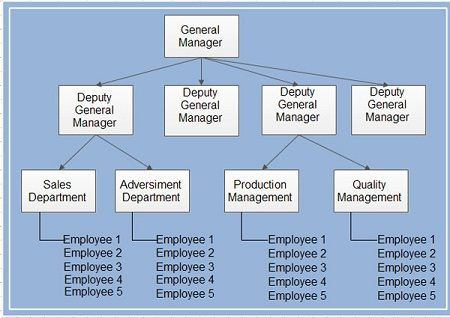
\includegraphics[width=\textwidth]{img/Hierarchical-Model.jpg}

        \column{0.5\textwidth}
            \centering
            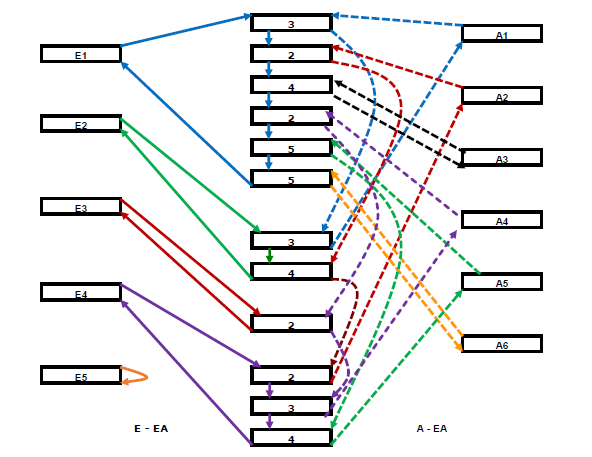
\includegraphics[width=\textwidth, height=0.8\textheight]{img/reticular.png}
    \end{columns}
\end{frame}




